\chapter{ピクセルモジュール}
この章ではピクセルモジュールの構成と各構成部品について説明する。

\section{ピクセルモジュールの構造}
ピクセルモジュールはベアモジュールとフレキシブル基板より構成される。
ベアモジュールは荷電粒子の通過を検知し、信号を発生するシリコンセンサーと、AD変換を行うFEチップで構成される。
ベアモジュールが持つFEチップの数はモジュールの種類によって異なる。
モジュールの構成を図\ref{module_configuration}に示す。

\begin{figure}[bpt]\centering
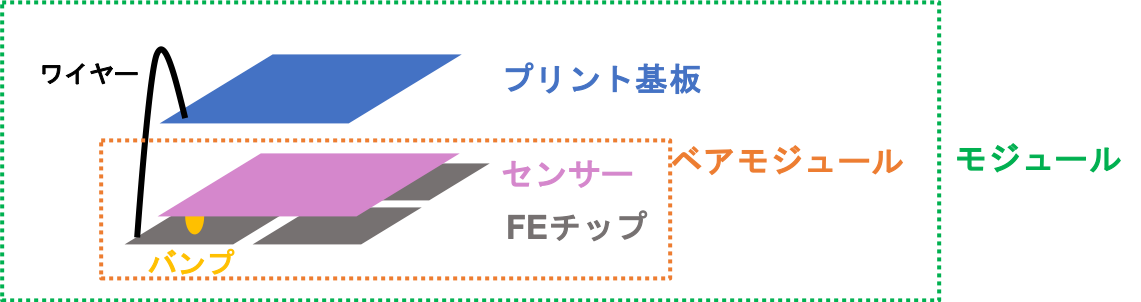
\includegraphics[width=14cm]{./module_configuration.png}
\caption[ピクセルモジュールの構成]{ピクセルモジュールの構成。図はQuadモジュールの構成を模式的に表したものである。モジュールは「\textbf{ベアモジュール}」と呼ばれる心臓部と「\textbf{フレキシブル基板}」を貼り付けることで作られる。ベアモジュールはセンサーとFEチップから成る。Quadモジュールの場合、1枚のセンサーに対しFEチップは4枚である。センサーとFEチップは「\textbf{バンプ}」と呼ばれる構造で電気的に接続しており、1ピクセルに対して1つのバンプ接合がなされている。FEチップとフレキシブル基板の接続には、ワイヤーが多数($O(100)$)配線される。}
\label{module_configuration}
\end{figure}

\section{ピクセルモジュールの構成部品}
\subsection{シリコンセンサー}
ピクセルモジュールに搭載するセンサーはシリコン半導体を用いている。
センサー内部構造としてpn接合を持ち、逆バイアス電圧をかけ空乏層を広げた状態で使用する\cite{2-1}。
この空乏層領域に荷電粒子が通過すると、Bethe-Blochの式\cite{2-3}に従い粒子はエネルギーを損失する。
このエネルギー損失量に従い、電子・ホール対が生成、これを収集することで荷電粒子の通過情報をアナログ信号として取得することができる。

新型ピクセルモジュールに搭載するセンサーは、n${}^+$ - in - p型である。
模式図を図\ref{sensor_image}に示す。$n^+$電極で電子を収集し、信号を取得する。
現行のセンサーに比べ、型変換を起こす可能性がなくなるため安定した運転が見込まれる\cite{1-3}。

\begin{figure}[bpt]\centering
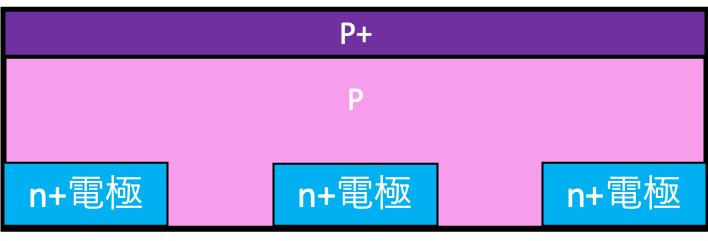
\includegraphics[width=8cm]{./sensor_image.png}
\caption[新型ピクセルモジュールに搭載するシリコンセンサーの断面図]{新型ピクセルモジュールに搭載するシリコンセンサーの断面図。図は新型ピクセルモジュールに搭載するシリコンセンサー断面の模式図を示している。p型半導体にn${}^+$型電極を埋め込んだn${}^+$ - in - p型と呼ばれる構造を持つ。p${}^+$側にフレキシブル基板、n${}^+$側にFEチップが付く。逆バイアス電圧を印加するとn${}^+$電極側から空乏層が広がる。}
\label{sensor_image}
\end{figure}

\subsection{読み出しFEチップ}
読み出しFEチップはシリコン半導体を用いて作られた集積回路である。
読み出しFEチップの主な役割は、シリコンセンサーで発生し受け取ったアナログ信号を整形、増幅したのちAD変換し、後段に転送することである。
AD変換について、アナログ信号がThresholdを超えた時間幅を測定し、デジタル信号に変換する。この信号の値を\textbf{Time over Threshold(ToT)}と呼ぶ。

ToTの概念図を図\ref{tot_algorithm}に示す。

\begin{figure}[bpt]\centering
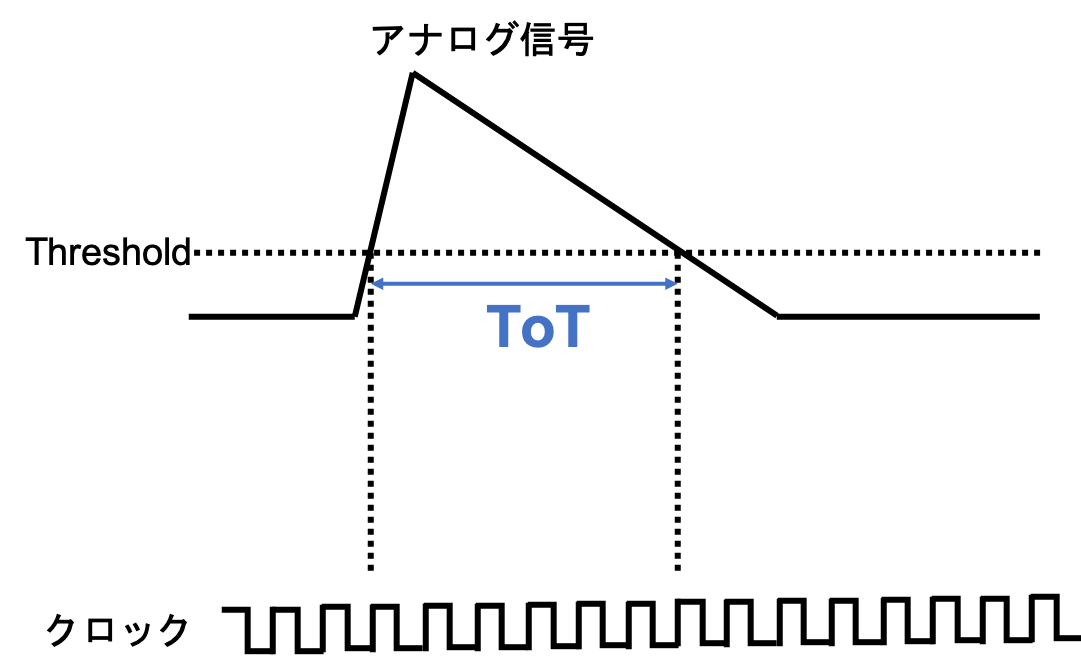
\includegraphics[width=10cm]{./tot_algorithm.png}
\caption[ToTの概念図]{ToTの概念図。FEチップで生成されるデジタル信号はToTと呼ばれる。図はその概念を模式的に表したものであり、FEチップで行われているAD変換である。ToTはアナログ信号がThreshold値を超えた時間幅に相当する。実際にはToT間のクロック数[b.c.]として取得さる。ここで1~b.c.(25~ns)はLHCにおける陽子の衝突間隔に相当する。}
\label{tot_algorithm}
\end{figure}

\subsubsection{RD53A}
RD53A\cite{2-1}は、新型ピクセルモジュールの研究、開発のために作られたプロトタイプの読み出しFEチップである。
RD53Aの性能を表\ref{rd53a_spec}に示す。
チップサイズ、ピクセル数は、ITkに搭載予定のモジュールが持つFEチップの半分となっている。

\begin{table}[tbp]
\begin{center}
\caption[RD53Aのスペック]{RD53Aのスペック。}
\label{rd53a_spec}
  \begin{tabular}{|ll|} \hline
    チップサイズ[mm$^2$] & $20.0\times 11.6$ \\ 
    ピクセルサイズ[$\mu$m$^2$] & $50.0\times 50.0$ \\ 
    ピクセル数[行$\times$列] & $400\times 192$ \\ 
    トリガーレート[kHz] & $1000$ \\ 
    データレート[Mbps] & $1280\times4$ \\ 
    ToTの範囲 & $0〜15$(4ビット) \\
    放射線耐性 & 500Mrad(トータルドーズ効果\cite{2-4}) \\\hline
  \end{tabular}
\end{center}
\end{table}

FEチップ上の各ピクセルはアナログ回路部とデジタル回路部を持つ。
RD53Aでは図\ref{fechip_rd53a}に示すように、3つの領域があり、それぞれの領域でピクセルのアナログ回路、AD変換回路が異なる。
左から順にSynchronous FE、Linear FE、Differrential FEと呼ぶ。
研究、開発用に3つの領域が設けられているが、性能比較の結果ITkに搭載するモジュールにはDifferrential FEを用いることが決定している。
なお、デジタル回路部は全てのピクセルにおいて共通である。
それぞれの回路図は付録\ref{chap:rd53a_circit}に示す。

\begin{figure}[bpt]\centering
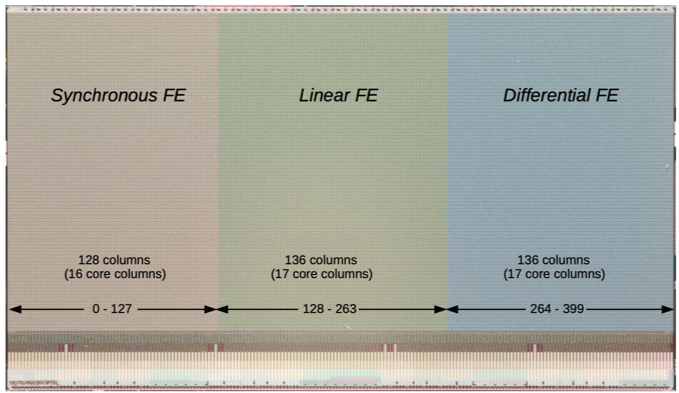
\includegraphics[width=10cm]{./fechip_rd53a.png}
\caption[RD53A]{RD53A\cite{2-1}。ピクセル数は400列$\times$192行となっている。図のようにRD53Aは3つの領域が設けられており、それぞれSynchronous FE、Linear FE、Differential FEと呼ぶ。各領域のピクセルが持つアナログ回路、AD変換回路が異なる。}
\label{fechip_rd53a}
\end{figure}

\subsection{フレキシブル基板}
フレキシブル基板は、基板上に電子部品が搭載されたものである。
FEチップからのデジタル信号を後段の回路へ転送する他、FEチップ、センサーへの電圧印加制御の役割も担う。

\subsection{信号伝達}
モジュールの信号伝達の様子を模式的に表したものを図\ref{module_electric_overview}に示す。
センサーで生成した信号はFEチップ、フレキシブル基板の順に送られ、PCでデータ取得できる。

\begin{figure}[bpt]\centering
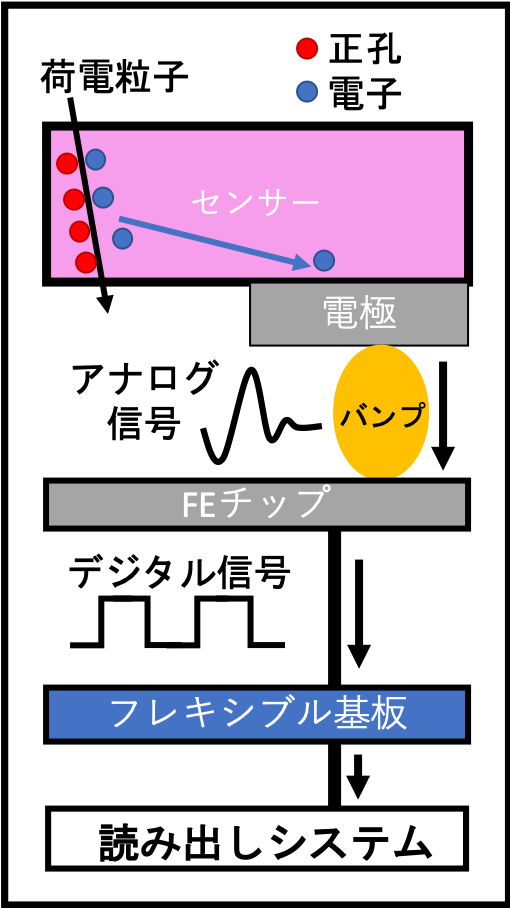
\includegraphics[width=6cm]{./module_electric_overview.png}
\caption[ピクセルモジュールにおける信号伝達の様子]{ピクセルモジュールにおける信号伝達の様子。図はピクセルモジュールにおける信号伝達の様子を模式的に表したものである。初めに、荷電粒子がセンサー部を通過し、エネルギー損失に応じた電子・ホール対を生成する。電子は電極により収集され、バンプを通してアナログ信号としてFEチップに送られる。FEチップでは信号を整形、増幅後、デジタル信号に変換する。その後ワイヤーを通してフレキシブル基板に転送、そしてPCに転送されデータを取得する。}
\label{module_electric_overview}
\end{figure}

\clearpage
\section{新型モジュールの種類}
現在、ITkに搭載するモジュールとして以下の3つのモジュールを予定している。
\begin{itemize}
  \item ステーブ用Tripletモジュール
  \item リング用Tripletモジュール
  \item Quadモジュール
\end{itemize}

Triplet、QuadモジュールはそれぞれFEチップを3、4枚搭載するモジュールである。
それぞれのモジュールの図及び検出器上における位置の一例を図\ref{module_geom}に示す。

\begin{figure}[bpt]\centering
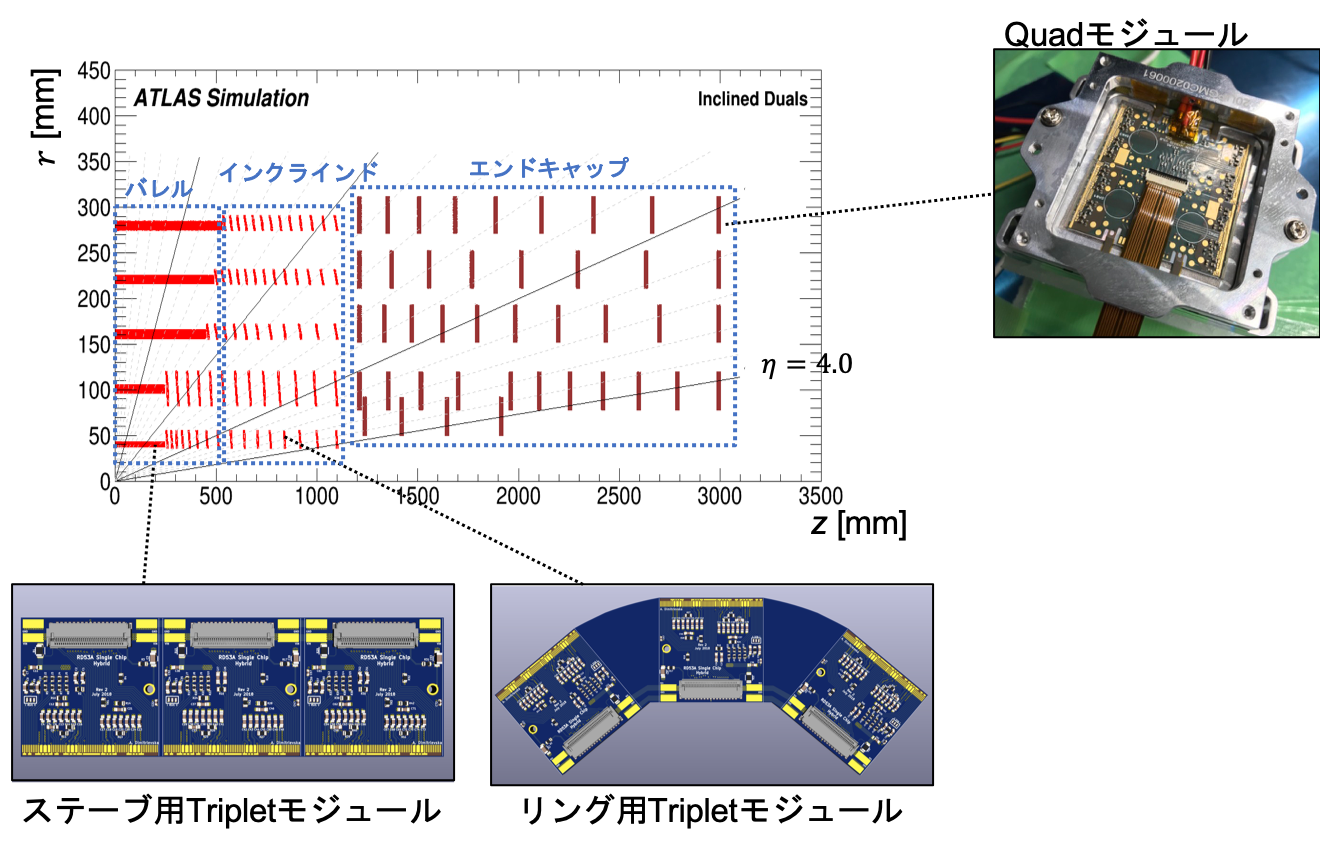
\includegraphics[width=12cm]{./module_geom.png}
\caption[搭載するモジュールのプロトタイプとITkにおける配置。]{搭載するモジュールのプロトタイプとITkにおける配置。2種類のTripletモジュールとQuadモジュールを搭載する予定となっている。Tripletモジュールは最内層のステーブ構造、リング構造の領域に使われる。それ以外の領域にはQuadモジュールが使われる。}
\label{module_geom}
\end{figure}


